\section{Color planes}
\begin{enumerate}[label=\emph{\alph*)}]
\item Swap the red and blue channels of the input image.
\begin{figure}[h!]
\centering
\begin{subfigure}{0.5\textwidth}
  \centering
  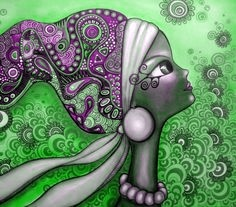
\includegraphics[width=0.5\linewidth]{../output/p0-2-a-0.jpg}
  \caption{Output for the input p0-1-0.jpg}
  \label{fig:sfig1}
\end{subfigure}%
\begin{subfigure}{0.5\textwidth}
  \centering
  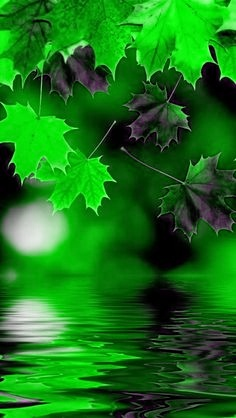
\includegraphics[width=0.5\linewidth]{../output/p0-2-a-1.jpg}
  \caption{Output for the input p0-1-1.jpg}
  \label{fig:sfig2}
\end{subfigure}
\begin{subfigure}{0.5\textwidth}
  \centering
  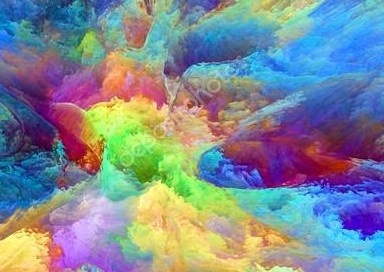
\includegraphics[width=0.5\linewidth]{../output/p0-2-a-2.jpg}
  \caption{Output for the input p0-1-2.jpg}
  \label{fig:sfig1}
\end{subfigure}%
\begin{subfigure}{0.5\textwidth}
  \centering
  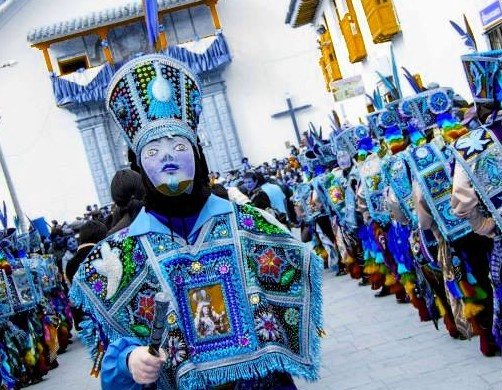
\includegraphics[width=0.5\linewidth]{../output/p0-2-a-3.jpg}
  \caption{Output for the input p0-1-3.jpg}
  \label{fig:sfig2}
\end{subfigure}
\caption{Output images for question 2.a}
\label{fig:fig}
\end{figure}
\\\\The imread() instruction of OpenCV reads images in format BGR, then we have to swap the channel blue(first channel) with the channel red(third channel), generating a new image in RGB format.\\We can see that the red colored regions become blue colored regions and the blue colored regions become  red colored regions\\

\item Create a monochrome image (img-green) by selecting the green channel of the input image.
\begin{figure}[h!]
\centering
\begin{subfigure}{0.5\textwidth}
  \centering
  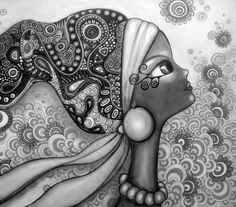
\includegraphics[width=0.5\linewidth]{../output/p0-2-b-0.jpg}
  \caption{Output for the input p0-1-0.jpg}
  \label{fig:sfig1}
\end{subfigure}%
\begin{subfigure}{0.5\textwidth}
  \centering
  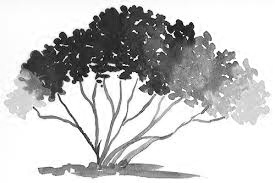
\includegraphics[width=0.5\linewidth]{../output/p0-2-b-1.jpg}
  \caption{Output for the input p0-1-1.jpg}
  \label{fig:sfig2}
\end{subfigure}
\begin{subfigure}{0.5\textwidth}
  \centering
  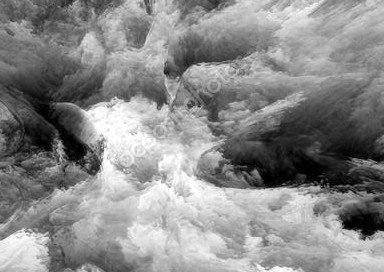
\includegraphics[width=0.5\linewidth]{../output/p0-2-b-2.jpg}
  \caption{Output for the input p0-1-2.jpg}
  \label{fig:sfig1}
\end{subfigure}%
\begin{subfigure}{0.5\textwidth}
  \centering
  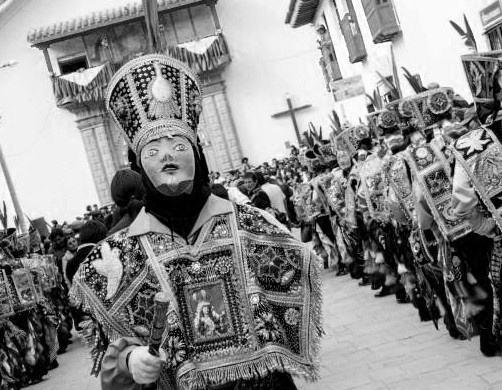
\includegraphics[width=0.5\linewidth]{../output/p0-2-b-3.jpg}
  \caption{Output for the input p0-1-3.jpg}
  \label{fig:sfig2}
\end{subfigure}
\caption{Output images for question 2.b}
\label{fig:fig}
\end{figure}
\\As we extract the green channel from the original image to generate a monochromatic image, then, the regions of the image that depend more on green color will have values close to 255 in the channel green, which means that in the output image those regions will have a color close to white, while the other regions of the image will have a color close to black.\\

\item Create a monochrome image (img-red) by selecting the red channel of the first input image.
\begin{figure}[h!]
\centering
\begin{subfigure}{0.5\textwidth}
  \centering
  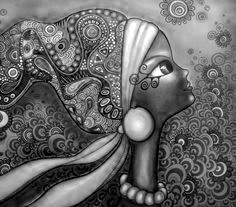
\includegraphics[width=0.5\linewidth]{../output/p0-2-c-0.jpg}
  \caption{Figura 13. Output for the input p0-1-0.jpg}
  \label{fig:sfig1}
\end{subfigure}%
\begin{subfigure}{0.5\textwidth}
  \centering
  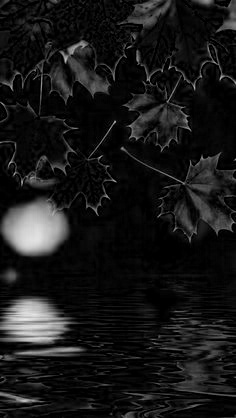
\includegraphics[width=0.5\linewidth]{../output/p0-2-c-1.jpg}
  \caption{Figura 14. Output for the input p0-1-1.jpg}
  \label{fig:sfig2}
\end{subfigure}
\begin{subfigure}{0.5\textwidth}
  \centering
  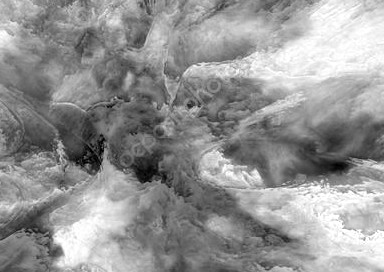
\includegraphics[width=0.5\linewidth]{../output/p0-2-c-2.jpg}
  \caption{Figura 15. Output for the input p0-1-0.jpg}
  \label{fig:sfig1}
\end{subfigure}%
\begin{subfigure}{0.5\textwidth}
  \centering
  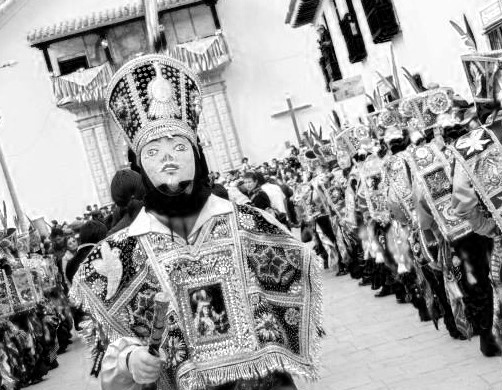
\includegraphics[width=0.5\linewidth]{../output/p0-2-c-3.jpg}
  \caption{Figura 16. Output for the input p0-1-1.jpg}
  \label{fig:sfig2}
\end{subfigure}
\caption{Output images for question 2.c}
\label{fig:fig}
\end{figure}
\\Similar to the previous interpretation, we say that the light colored regions in the output image are red colored regions in the original image.\\
\item Which image looks more like what you would expect a monochrome image to look like? Would you
expect a computer vision algorithm to work on one better than the other? Why?
\begin{enumerate}[label=\arabic*)]
\item The monoch	rome image generated from the green channel is the image that most closely resembles the monochrome image that I would expect from the original image.
\item I think that in computer vision, the computing power of a computer is more important than the optimization of an algorithm, because in computer vision we work on the representation of an image, which is an matrix, then to perform any type of operation in a Matrix we will need to go through this in any way. \\In conclusion one algorithm works better than another depending on the environment in which it is executed.
\end{enumerate}
\end{enumerate}
